\section{Einführung}
\label{sec:einfuehrung}

Besonders in sehr dynamischen Forschungsbereichen, wie beispielsweise dem Machine Learning, ist es wichtig, stets auf dem aktuellen Stand der Forschung zu bleiben.
Dies ist jedoch aufgrund der hohen Anzahl an wissenschaftlichen Publikationen, die jährlich veröffentlicht werden \cite{scientific-growth}, eine Herausforderung; herkömmliche Literaturübersichten können bereits nach wenigen Monaten überholt sein.
Eine Möglichkeit, um den Überblick zu behalten, sind sogenannte \textit{Living Literature Reviews} (LLRs).
Diese werden regelmäßig aktualisiert und enthalten eine Zusammenfassung der aktuellen Forschungsergebnisse zu einem bestimmten Thema.

In der vorliegenden Arbeit wird zuerst der Anwendungsfall näher erläutert.
Anschließend werden zwei Ansätze zur Erstellung und Aktualisierung von LLRs vorgestellt und miteinander verglichen:
\textit{Genuine Semantic Publishing} \cite{kuhn2017genuine}, beruhend auf von den Autoren selbst erstellten und veröffentlichten, maschinenverarbeitbaren Informationen über Ihre Forschungsbeiträge, und \textit{SCICERO}, ein auf Natural Language Processing und Transformer-Modellen beruhender Ansatz.
Dabei wird untersucht, wie gut die beiden Ansätze in der Lage sind, den Anforderungen des intendierten Anwendungsszenarios gerecht zu werden und welche Vor- und Nachteile sie haben.

\begin{figure}[bhp]
    \centering
    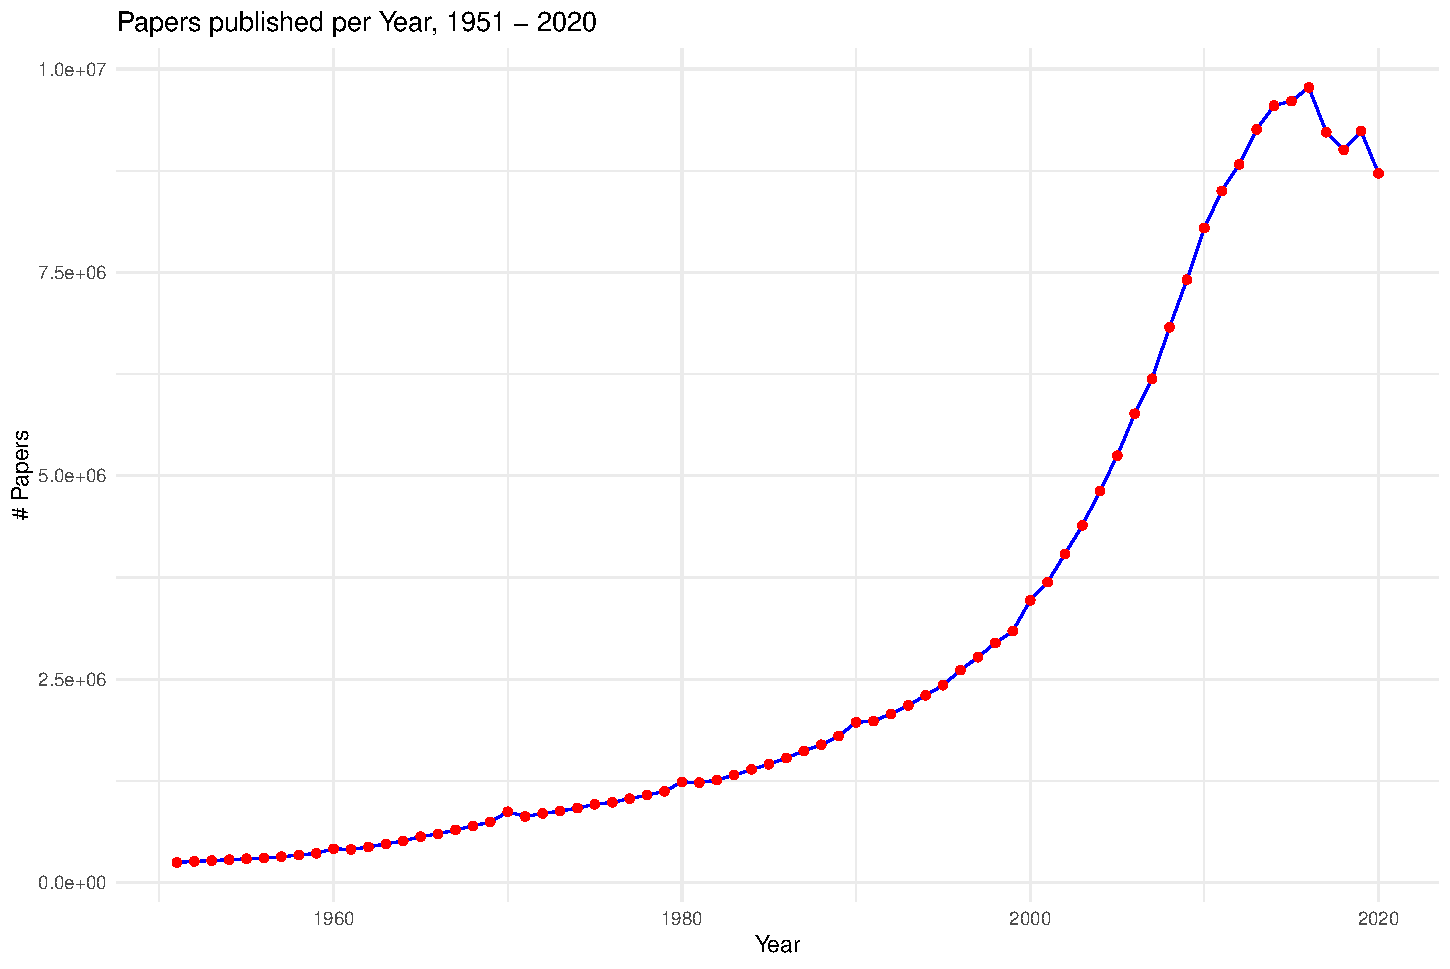
\includegraphics[width=0.5\textwidth]{figures/papers-per-year.pdf}
    \caption{Anzahl der jährlich veröffentlichten wissenschaftlichen Publikationen, 1951-2020. Eigene Darstellung nach Daten von \citet{papers-per-year}.}
    \label{fig:overview}
\end{figure}
